\chapter*{CAPÍTULO I: MEMORIA DESCRIPTIVA}
\addcontentsline{toc}{chapter}{CAPÍTULO I: MEMORIA DESCRIPTIVA}

\section{GENERALIDADES Y ANTECEDENTES}

El presente Expediente Técnico de Ingeniería ha sido elaborado para el dimensionamiento, diseño y especificación electromecánica del proyecto: \textbf{``Electrificación y Redes de Distribución en Media Tensión (10 kV) y Baja Tensión (380/220 V) desde la Minicentral Hidroeléctrica Limbani (200 kW, Turbina Michell-Banki)''}, ubicado en el distrito de Limbani, provincia de Sandia, departamento de Puno.

Históricamente, los centros poblados y distritos situados en las vertientes orientales de la cordillera de Carabaya y Sandia han enfrentado limitaciones en el suministro continuo y de calidad de energía eléctrica, debido a la topografía accidentada y la lejanía de las grandes troncales del Sistema Eléctrico Interconectado Nacional (SEIN). En este contexto, el aprovechamiento del abundante potencial hídrico de la cuenca del Río Limbani mediante la operación de una minicentral hidroeléctrica de pasada con turbina Michell-Banki de 200 kW representa una solución técnica, económica y ambientalmente sostenible para garantizar la soberanía energética del casco urbano de Limbani.

Para la concepción del presente proyecto se ha tomado como base territorial y física el \textbf{Catastro Urbano Oficial Consolidado de Limbani}, levantado en el sistema geodésico WGS 84 / UTM Zona 19 Sur, el cual registra con precisión milimétrica un total de \textbf{587 lotes catastrados de propiedad oficial y 87 manzanas urbanas}, así como la delimitación inalterable del cauce del Río Limbani, Río Chinchalamani y los equipamientos urbanos (Plaza de Armas, Estadio Municipal, Piscina y centros educativos/salud).

\section{UBICACIÓN POLÍTICA, GEOGRÁFICA Y ACCESIBILIDAD}

\subsection{Ubicación Política}
\begin{itemize}
  \item \textbf{Departamento:} Puno
  \item \textbf{Provincia:} Sandia
  \item \textbf{Distrito:} Limbani
  \item \textbf{Sector beneficiario:} Casco urbano consolidado (Barrio Norte, Centro Urbano y Barrio Sur)
\end{itemize}

\subsection{Ubicación Geográfica y Topográfica}
El distrito de Limbani se emplaza en una garganta y valle encajonado de alta pendiente en la vertiente oriental andina:
\begin{itemize}
  \item \textbf{Altitud media:} 3,050 m.s.n.m. (rango entre 2,980 m.s.n.m. en la salida sur y 3,150 m.s.n.m. en la captación norte).
  \item \textbf{Coordenadas UTM (WGS 84 Zona 19 Sur):}
    \begin{itemize}
      \item Este: 425,250 m E a 425,700 m E
      \item Norte: 8'434,750 m N a 8'436,650 m N
    \end{itemize}
\end{itemize}

\subsection{Alcance y Objeto del Proyecto}
Se precisa que las características técnicas de la Minicentral Hidroeléctrica Limbani (turbina hidráulica tipo Michell-Banki de 200 kW y alternador síncrono trifásico a 380 V) constituyen \textbf{parámetros de entrada de generación y punto de partida del suministro eléctrico}. El alcance específico y objeto integral del presente Expediente Técnico de Ingeniería de Detalle comprende:
\begin{enumerate}
  \item El diseño electromecánico de la \textbf{Subestación Elevadora} en casa de máquinas ($250\text{ kVA}$, $0.38 / 10.0\text{ kV}$).
  \item La traza, cálculo y diseño de la \textbf{Línea Primaria en Media Tensión (10.0 kV)}, de $1,967.87\text{ m}$ ($1.97\text{ km}$) de longitud en conductor desnudo AAAC $35\text{ mm}^2$ sobre postería de concreto armado centrifugado (CAC) de 12 m y 13 m.
  \item El dimensionamiento y ubicación física de las \textbf{tres (03) Subestaciones Aéreas Biposte (SAB)}: SED-01 (50 kVA), SED-02 (100 kVA) y SED-03 (100 kVA).
  \item El trazado y cálculo de las \textbf{Redes Secundarias de Distribución en Baja Tensión (380/220 V)} con $6,206.73\text{ m}$ de cables autoportantes tipo CAAI, soportadas en 243 postes CAC de 8m y 9m estrictamente ubicados en la trama urbana consolidada.
  \item El sistema de \textbf{Alumbrado Público LED} con 166 luminarias de 50 W y control fotocelular.
  \item Las \textbf{587 Acometidas Domiciliarias} (534 cortas $\le 15\text{ m}$ y 53 largas $15-30\text{ m}$) con cable concéntrico SET $2\times 4\text{ mm}^2$, cajas de policarbonato L-T, medición de energía estática e interruptores de protección.
\end{enumerate}

\subsection{Cartografía e Ilustraciones de Ubicación Territorial}

A continuación se ilustra la localización político-geográfica en tres niveles de escala (macro, meso y microregional):

\begin{figure}[H]
\centering
\begin{minipage}{0.48\textwidth}
  \centering
  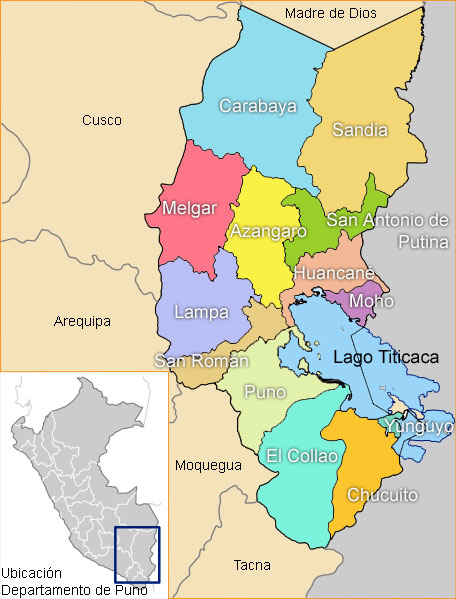
\includegraphics[width=\textwidth,height=0.28\textheight,keepaspectratio]{figuras/ubicacion_departamento_puno.jpg}
  \caption{Ubicación de la Provincia de Sandia en el Departamento de Puno.}
  \label{fig:puno_politico}
\end{minipage}\hfill
\begin{minipage}{0.48\textwidth}
  \centering
  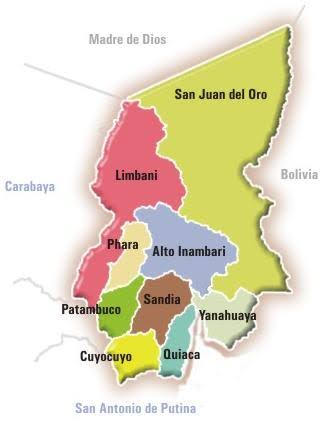
\includegraphics[width=\textwidth,height=0.28\textheight,keepaspectratio]{figuras/ubicacion_provincia_sandia.jpg}
  \caption{Mapa de la Provincia de Sandia y acceso vial al Distrito de Limbani.}
  \label{fig:sandia_provincia}
\end{minipage}
\end{figure}

\begin{figure}[H]
\centering
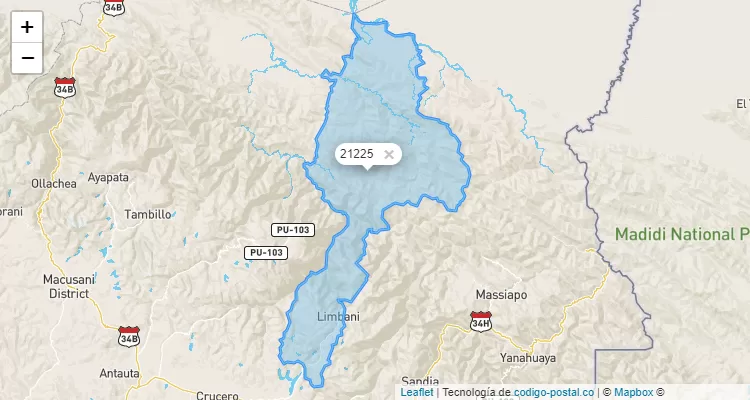
\includegraphics[width=0.85\textwidth,height=0.25\textheight,keepaspectratio]{figuras/ubicacion_macrorregional.png}
\caption{Localización orográfica y relieve del Distrito de Limbani en la vertiente oriental andina.}
\label{fig:limbani_relieve}
\end{figure}

\subsection{Vías de Acceso}
El acceso al distrito de Limbani desde la capital departamental se realiza mediante el siguiente itinerario vial terrestre:
\begin{table}[H]
\centering
\small
\begin{tabular}{|l|l|c|l|c|}
\hline
\textbf{Tramo} & \textbf{Tipo de Vía} & \textbf{Distancia (km)} & \textbf{Estado} & \textbf{Tiempo (h)} \\
\hline
Puno -- Juliaca & Asfaltada (Red Nacional) & 44.0 & Bueno & 0.8 h \\
Juliaca -- Huancané -- Ananea & Asfaltada / Afirmada & 128.0 & Regular & 2.5 h \\
Ananea -- Crucero -- Limbani & Afirmada / Trocha afirmada & 62.0 & Tránsito moderado & 2.2 h \\
\hline
\multicolumn{2}{|r|}{\textbf{Total Itinerario Terrestre}} & \textbf{234.0 km} & \multicolumn{2}{r|}{\textbf{$\approx$ 5.5 horas}} \\
\hline
\end{tabular}
\caption{Ruta de acceso terrestre a la zona del proyecto.}
\end{table}

\section{CONDICIONES AMBIENTALES Y CLIMATOLÓGICAS}

Conforme a la zonificación bioclimática y la Parte 2 del Código Nacional de Electricidad - Suministro 2011 (Zona 2: Sierra y Altiplano):
\begin{itemize}
  \item \textbf{Temperatura mínima extrema:} $-5.0\ ^\circ\text{C}$ (noches de helada invernal).
  \item \textbf{Temperatura media anual:} $+12.0\ ^\circ\text{C}$.
  \item \textbf{Temperatura máxima extrema:} $+35.0\ ^\circ\text{C}$ (radiación solar directa diurna).
  \item \textbf{Velocidad máxima de viento de diseño:} $90.0\text{ km/h}$ ($25.0\text{ m/s}$).
  \item \textbf{Precipitación pluvial media:} $850\text{ mm/año}$ (temporada de lluvias concentrada entre diciembre y marzo).
  \item \textbf{Nivel ceráunico (días de tormenta al año):} 60 a 75 días de tormenta/año (nivel medio-alto, requiere protección con pararrayos en todas las SED y finales de línea).
  \item \textbf{Resistividad aparente del terreno:} Terreno rocoso y arcillo-arenoso variable entre $150\ \Omega\cdot\text{m}$ y $450\ \Omega\cdot\text{m}$.
\end{itemize}

\section{DESCRIPCIÓN DE LA FUENTE DE GENERACIÓN: MCH LIMBANI}

La energía base del sistema proviene de la \textbf{Minicentral Hidroeléctrica Limbani (MCH Limbani)}, cuyas características técnicas principales son:
\begin{itemize}
  \item \textbf{Tipo de central:} Central hidroeléctrica de pasada con derivación de caudal del Río Limbani.
  \item \textbf{Turbina hidráulica:} Tipo \textbf{Michell-Banki} (flujo transversal o cross-flow). La selección de esta máquina obedece a su excelente curva de rendimiento ante fluctuaciones de caudal estacional y su robustez ante aguas de montaña con arrastre de sedimentos finos.
  \item \textbf{Potencia mecánica en eje:} $\approx 220\text{ kW}$ ($295\text{ HP}$).
  \item \textbf{Generador eléctrico:} Generador sincrónico trifásico sin escobillas (brushless), 4 polos, $1,800\text{ RPM}$, $60\text{ Hz}$.
  \item \textbf{Potencia eléctrica nominal:} $200.0\text{ kW}$ ($250.0\text{ kVA}$ con $\cos\phi = 0.80$).
  \item \textbf{Tensión en bornes de generación:} $380\text{ V}$ ($0.38\text{ kV}$) trifásico.
  \item \textbf{Subestación Elevadora de Central:} Ubicada en la casa de máquinas en el extremo norte urbano (coordenadas UTM $E=425,580$, $N=8'436,580$). Consta de un transformador elevador trifásico de $250\text{ kVA}$, relación de transformación $0.38 / 10.0\text{ kV}$, grupo de conexión Dyn5, en baño de aceite mineral dieléctrico.
\end{itemize}

\section{ALCANCE Y DESCRIPCIÓN DEL SISTEMA ELÉCTRICO PROPUESTO}

El proyecto contempla tres subsistemas eléctricos integrados e interdependientes:

\begin{figure}[H]
\centering
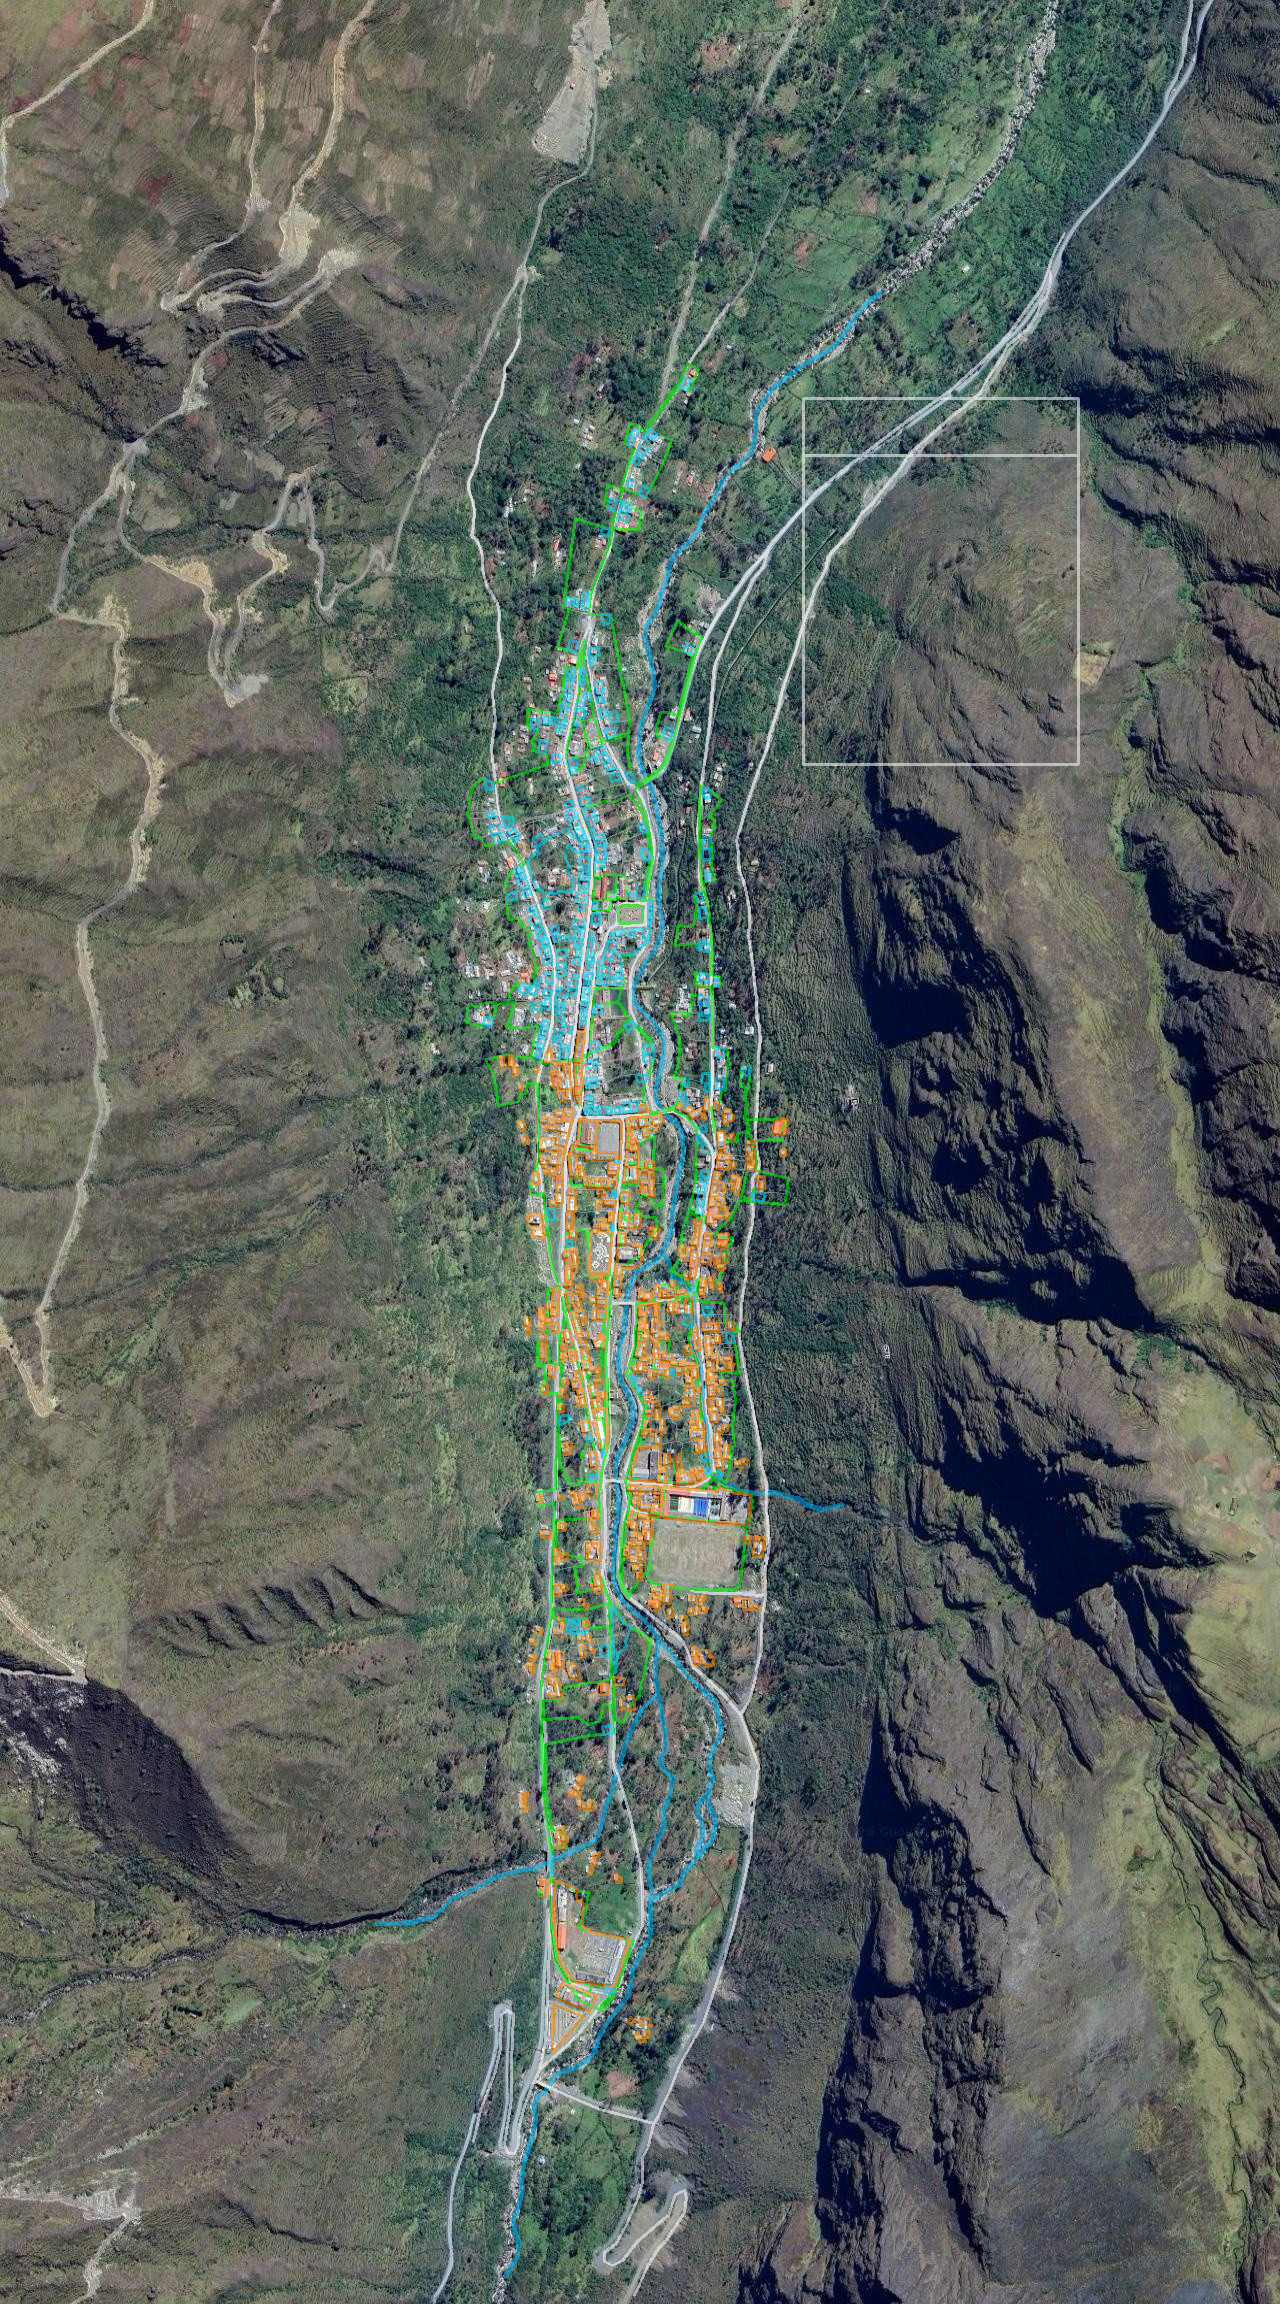
\includegraphics[width=0.88\textwidth]{figuras/01_superposicion_ortofoto_completa.png}
\caption{Vista general de superposición del catastro urbano oficial de Limbani sobre ortofoto satelital, base para el trazado de redes.}
\end{figure}

\subsection{Línea Primaria en Media Tensión (10 kV)}
\begin{itemize}
  \item \textbf{Tensión nominal:} $10.0\text{ kV}$ trifásico, 3 hilos, $60\text{ Hz}$.
  \item \textbf{Tensión máxima de diseño:} $12.0\text{ kV}$.
  \item \textbf{Longitud total de trazo troncal:} $2.15\text{ km}$, recorriendo de norte a sur a lo largo de las vías y franjas de servidumbre urbana, sin cruces sobre el cauce activo de los ríos.
  \item \textbf{Conductor seleccionado:} Conductor desnudo de aleación de aluminio tipo \textbf{AAAC de 35 mm$^2$} (NTP 370.258).
  \item \textbf{Soportes y estructuras:} Postes de Concreto Armado Centrifugado (CAC) de $12\text{ m}/300\text{ daN}$ para alineamiento y $13\text{ m}/400-600\text{ daN}$ para ángulos y anclajes, con crucetas de acero galvanizado en caliente de $2.0\text{ m}$ y aisladores poliméricos tipo pin (ANSI 56-3) y suspensión (ANSI 52-3).
\end{itemize}

\subsection{Subestaciones de Distribución (SED)}
Para abastecer de forma balanceada a los 587 predios y mantener caídas de tensión inferiores al $5\%$ en baja tensión, se han zonificado \textbf{tres (03) Subestaciones Aéreas Biposte (SAB)}:

\begin{table}[H]
\centering
\small
\begin{tabular}{|l|c|c|l|c|}
\hline
\textbf{Código SED} & \textbf{Potencia} & \textbf{Relación (kV)} & \textbf{Zona Urbana de Cobertura} & \textbf{Lotes} \\
\hline
\textbf{SED-01 (Norte)} & 50 kVA & 10.0 / 0.38-0.22 & Barrio Norte, Central Hidroeléctrica, Jr. Villa Hermosa & 112 \\
\textbf{SED-02 (Centro)} & 100 kVA & 10.0 / 0.38-0.22 & Plaza de Armas, Jr. Progreso, Jr. Lima, Comercio, Salud & 268 \\
\textbf{SED-03 (Sur)} & 100 kVA & 10.0 / 0.38-0.22 & Barrio Sur, Estadio Municipal, Piscina, Recreación & 207 \\
\hline
\multicolumn{2}{|r|}{\textbf{Total Capacidad de Transformación}} & \textbf{250 kVA} & \textbf{Cobertura Casco Urbano Consolidado} & \textbf{587 lotes} \\
\hline
\end{tabular}
\caption{Distribución y características técnicas de las Subestaciones de Distribución (SED).}
\end{table}

\subsection{Redes de Distribución Secundaria en Baja Tensión (380/220 V)}
\begin{itemize}
  \item \textbf{Sistema de distribución:} Trifásico tetrafilar con neutro múltiplemente puesto a tierra: $380/220\text{ V}$, $60\text{ Hz}$.
  \item \textbf{Tensión de suministro domiciliario:} $220\text{ V}$ monofásico entre fase y neutro.
  \item \textbf{Conductor autoportante:} Cable aéreo autoportante de aluminio aislado con polietileno reticulado (XLPE) tipo \textbf{CAAI}:
    \begin{itemize}
      \item Circuitos troncales ($3,980.15\text{ m}$): $\text{CAAI } 3\times 35 + 1\times 16 + \text{NA } 25\text{ mm}^2$.
      \item Circuitos ramales ($2,226.57\text{ m}$): $\text{CAAI } 2\times 16 + 1\times 16 + \text{NA } 25\text{ mm}^2$.
    \end{itemize}
  \item \textbf{Postes de baja tensión:} 243 postes de concreto armado centrifugado CAC de $8\text{ m}/200\text{ daN}$ (66 unid), $8\text{ m}/300\text{ daN}$ (38 unid) y $9\text{ m}/300\text{ daN}$ (139 unid), circunscritos exclusivamente al área urbana poblada.
\end{itemize}

\subsection{Sistema de Alumbrado Público (AP)}
\begin{itemize}
  \item Instalación de 166 luminarias LED para alumbrado público de $50\text{ W}$, flujo luminoso nominal de $6,500\text{ lm}$, con fotocélula electrónica individual y brazo pastoral de acero galvanizado montado sobre los postes de la red secundaria conforme a la R.D. N° 017-2003-EM/DGE.
\end{itemize}

\section{BASE LEGAL Y NORMATIVA TÉCNICA PERUANA}

El desarrollo íntegro del proyecto se sustenta en el marco regulatorio vigente:
\begin{enumerate}
  \item \textbf{Código Nacional de Electricidad - Suministro 2011 (R.M. N.° 366-2011-MEM/DM):} Cumplimiento estricto de distancias mínimas de seguridad, esfuerzos mecánicos de postes y conductores, retenidas mecánicas (Regla 261) y puesta a tierra.
  \item \textbf{Ley de Concesiones Eléctricas (D.L. N.° 25844)} y su Reglamento (D.S. N.° 009-93-EM).
  \item \textbf{Ley General de Electrificación Rural (Ley N.° 28749)} y su Reglamento (D.S. N.° 025-2007-EM).
  \item \textbf{Norma DGE R.D. N.° 018-2003-EM/DGE:} Bases para el Diseño de Líneas Primarias para Electrificación Rural.
  \item \textbf{Norma DGE R.D. N.° 016-2003-EM/DGE:} Bases para el Diseño de Redes Secundarias con Conductores Autoportantes.
  \item \textbf{Norma DGE R.D. N.° 024-2003-EM/DGE:} Soportes Normalizados para Líneas y Redes Primarias para Electrificación Rural.
  \item \textbf{Norma DGE R.D. N.° 023-2003-EM-DGE:} Soportes Normalizados para Líneas y Redes Secundarias para Electrificación Rural.
  \item \textbf{Norma DGE R.D. N.° 017-2003-EM/DGE:} Alumbrado de Vías Públicas en Áreas Rurales.
  \item \textbf{Norma DGE R.D. N.° 026-2003-EM/DGE:} Especificaciones Técnicas para el Montaje de Líneas y Redes.
  \item \textbf{Norma Técnica de Calidad de los Servicios Eléctricos - NTCSE (D.S. N.° 020-97-EM):} Tolerancia máxima de tensión admisible de $\pm 5.0\%$ en barra de MT y bornes de usuario.
  \item \textbf{Norma DGE R.M. N.° 091-2002-EM/VME:} Símbolos Gráficos en Electricidad (Sección 9: Retenidas, Puestas a Tierra y Postería).
\end{enumerate}
